\documentclass{beamer}
\usepackage[T1]{fontenc}
\usepackage{graphicx}
\usepackage{tikz}
\usepackage{tikzducks}
\usepackage{xcolor}
\usepackage{amsmath}
\usetikzlibrary{calc}

\definecolor{ted}{HTML}{E62B1E}

\usetheme{Szeged}
\usecolortheme{whale}
\setbeamercolor{palette primary}{bg=violet!80!black,fg=white}
\setbeamercolor{palette secondary}{bg=violet!60!black,fg=white}
\setbeamercolor{palette tertiary}{bg=violet!40!black,fg=white}
\setbeamercolor{palette quaternary}{bg=violet!20!black,fg=white}
\setbeamercolor{structure}{fg=violet!60!black}

\setbeamertemplate{background}%
{%
    \begin{tikzpicture}[remember picture,overlay]{\node[yshift=1.5cm,xshift=-2cm,opacity=0.1] at (current page.south east)
      {
      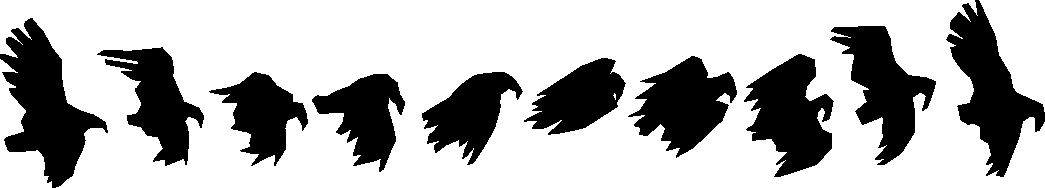
\includegraphics[scale=0.4, angle=25]{ptaki.pdf}
      }
      ;
    \node[yshift=-2cm,xshift=-2cm,opacity=0.05] at (current page.north east)
      {
      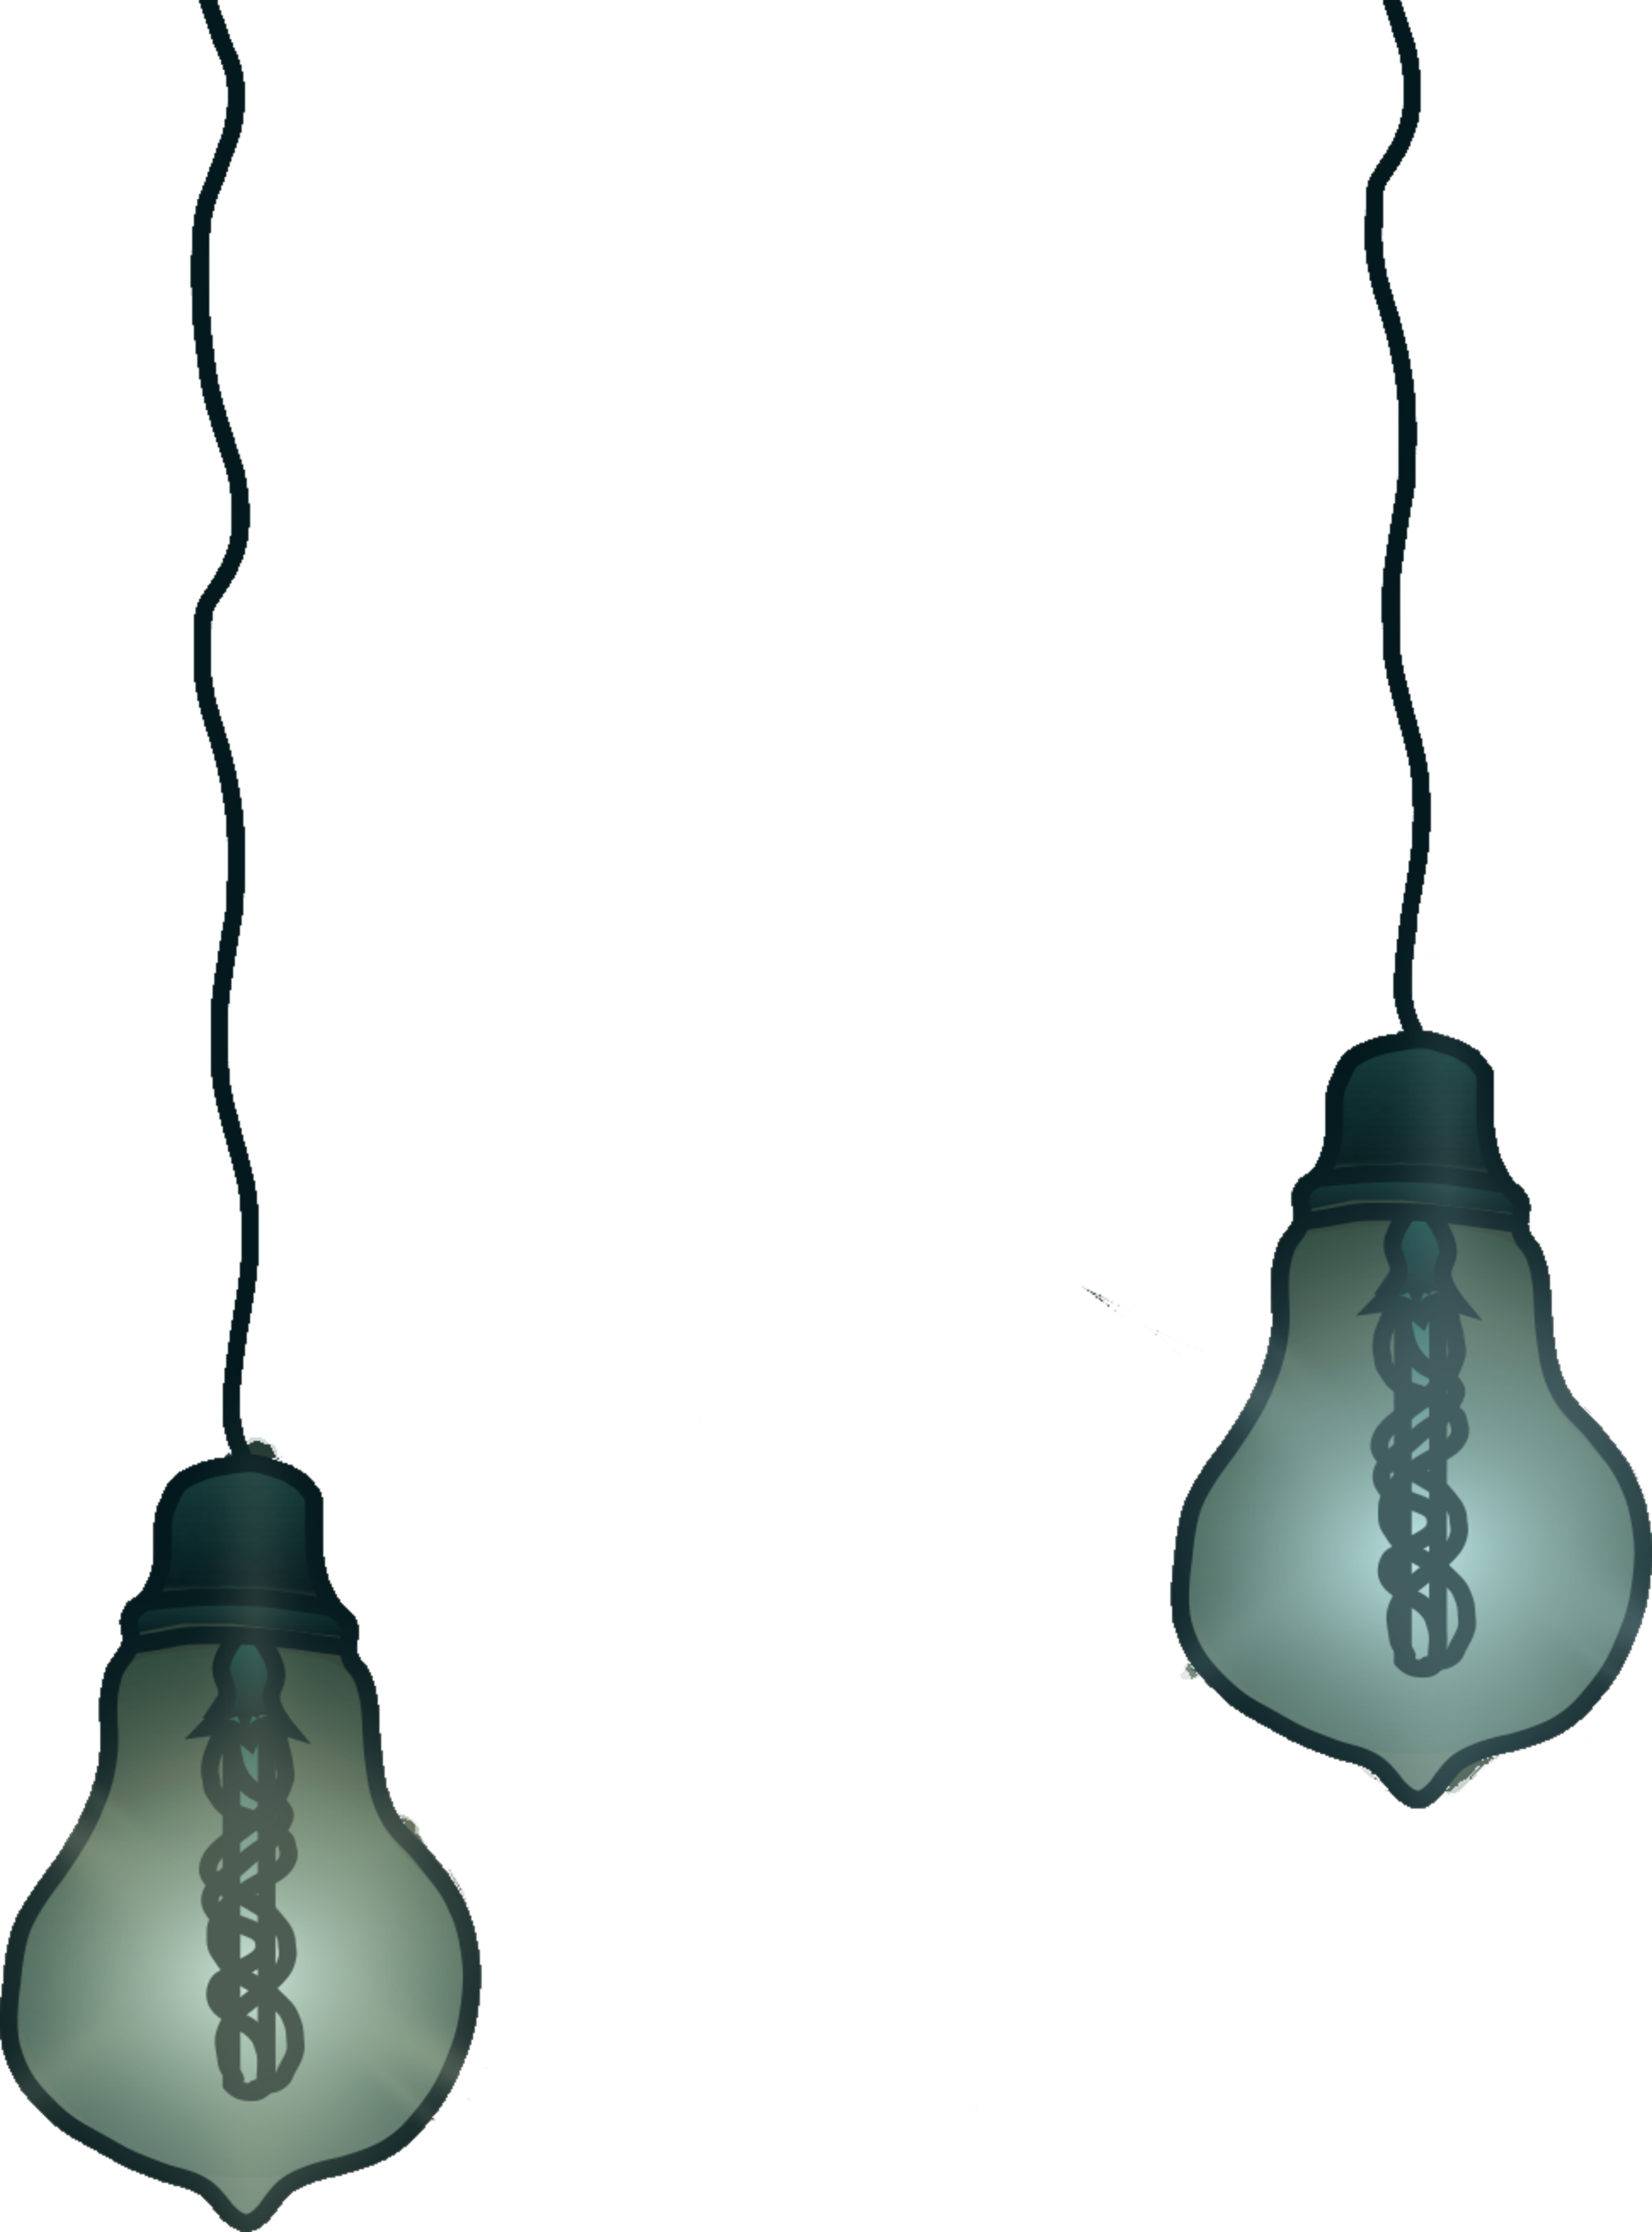
\includegraphics[scale=0.1, angle=0]{zarowki.pdf}
      }
      ;
    % \node[yshift=1.0cm,xshift=0.6cm] (logopos) at (current page.south west) {{\begin{tikzpicture}\shuffleducks\duck[signpost=\insertframenumber, \randomhead,scale=.4]\end{tikzpicture}}};
    % \pgfmathsetmacro{\progress}{360*(\insertframenumber)/(\inserttotalframenumber)}%;
    % \draw[line width=0.2*3pt] ([xshift=0.55cm] logopos)  arc[radius=0.55cm, start angle=0, end angle=\progress];
    % \fill ([shift={(\progress:0.55cm)}] logopos) circle(1pt);

    }
        \end{tikzpicture}
    
}

\title{Hydrodynamika ludzi, czyli dlaczego ludzie nie zderzają się ze sobą}
\institute{Mateusz ''{\color{black}\(\blacksquare\)}'' Winiarski}

\begin{document}

\newsavebox{\langevinbox}
\sbox{\langevinbox}{%
  \begin{minipage}{0.6\linewidth}% adjust width as needed
    \hfill równania Langevina, \(n=1\): \hfill~
    \[
    \begin{cases}
      \frac{dx}{dt} &= u(t) \\
      \frac{dy}{dt} &= v(t) \\
      \frac{du}{dt} &= -4\alpha_i u \bigl(u^2 - u_{p,i}^2\bigr) + \sigma_x \dot{W}_x \\
      \frac{dv}{dt} &= -2\nu v(t) - 2\beta (y - y_p) + \sigma_y \dot{W}_y
    \end{cases}
    \]
  \end{minipage}%
}
\newsavebox{\myduckbox}
\sbox{\myduckbox}{%
    
\begin{tikzpicture}
        \duck[water=blue,sunglasses,crazyhair=black!50!gray,tshirt=cyan]
    \end{tikzpicture}%
}

\begin{frame}{}{}
% \begin{figure}
%  \centering
% \tikzset{ampersand replacement=\&}
\begin{tikzpicture}[remember picture,overlay]
 \node[anchor=north west, xshift=-1cm] (ted) at (current page.north west) {
\includegraphics[width=0.5\textwidth]{images/2026-06-10-21-09-10.png}};
 \node[anchor=west] at ($(ted.east)+(-1.3cm,0.2cm)$) {\Huge \bfseries \rmfamily \color{ted} \TeX};

 \node[anchor=south west] at (current page.south west) {
\includegraphics[width=0.8\textwidth]{images/2025-11-13-13-52-03.png}};

 \node[anchor=north east] (ein) at ($(current page.north east) + (0,-1cm)$) {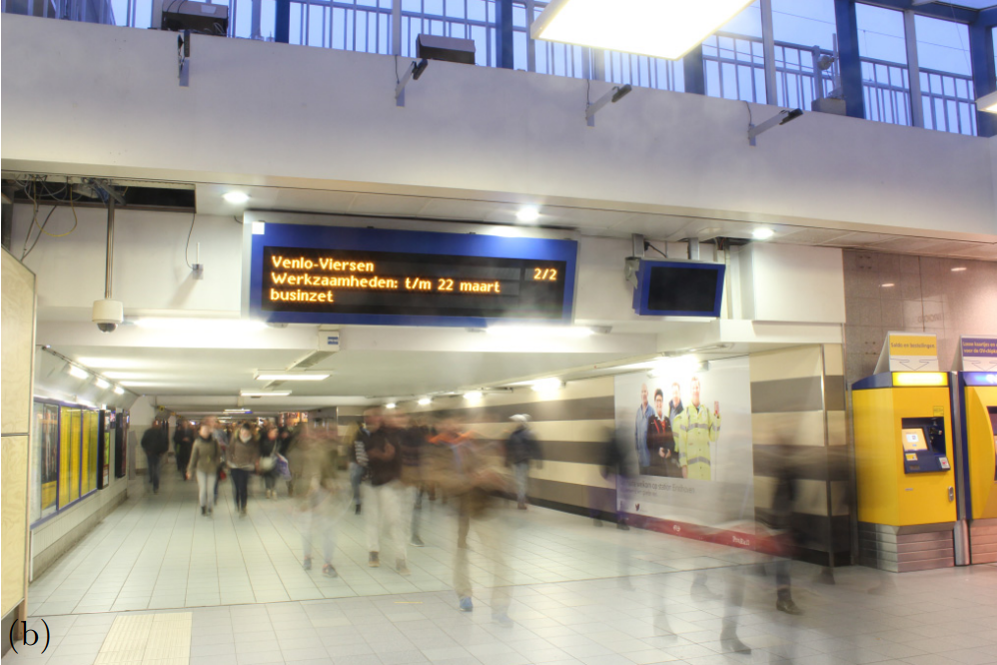
\includegraphics[width=0.6\textwidth]{images/2025-11-13-14-23-37.png}};
 \node[anchor=south] at ($(ein.south)+(0,-0.4cm)$) {dworzec w Eindhoven};

 \node[anchor=south] at ($(ted.south)+(-0.3cm,-3.2cm)$) {
  równania Langevina: \usebox{\langevinbox}
 };
\node[anchor=south east, xshift=-2mm, yshift=2mm] at (current page.south east) {\usebox{\myduckbox}};

%  \caption{}
%  \end{figure}
\end{tikzpicture}


\end{frame}


\begin{frame}{}{}
  
\transglitter

\begin{tikzpicture}[remember picture,overlay]
 \node[anchor=north west, xshift=0cm, yshift=-0.7cm] (led) at (current page.north west) {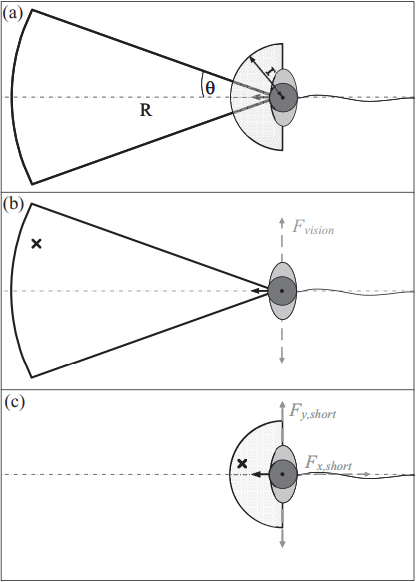
\includegraphics[width=0.5\textwidth]{images/2025-11-13-19-12-20.png}};
 \node[anchor=north] at ($(led.north)+(-1.2cm,-3.5cm)$) {\small $F_{vision}\sim \exp\left(-\frac{d^2}{R^2}\right)$};
 \node[anchor=north] at ($(led.north)+(-1.2cm,-5.8cm)$) {\small $F_{short}\sim \exp\left(-\frac{d^2}{r^2}\right)$};

%  \node[anchor=south west] at (current page.south west) {
\includegraphics[width=0.8\textwidth]{images/2025-11-13-13-52-03.png}};

 \node[anchor=north east] (ein) at ($(current page.north east) + (0cm,-0.5cm)$) { 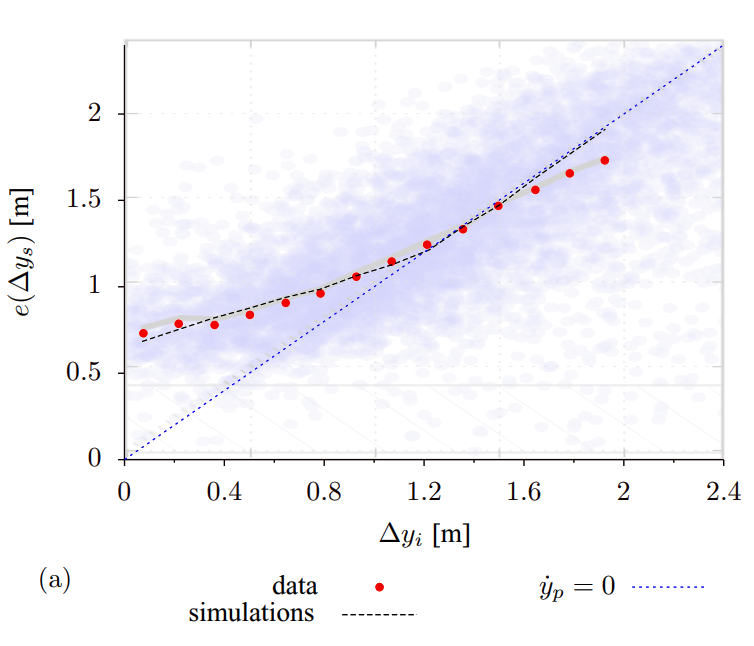
\includegraphics[width=0.4\textwidth]{images/2026-06-11-01-20-21.png}};
  \node[anchor=north, font=\small] at ($(ein.south)+(0.3cm,+1.1cm)$) {położenie $\Delta y$ na wejściu};
 \node[anchor=east, font=\small, rotate=90] at ($(ein.west)+(+0.0cm,+1.8cm)$) {położenie $\Delta y$ w mijaniu};

  \node[anchor=north] (zwei) at ($(ein.south) + (-2.0cm,0.5cm)$) { 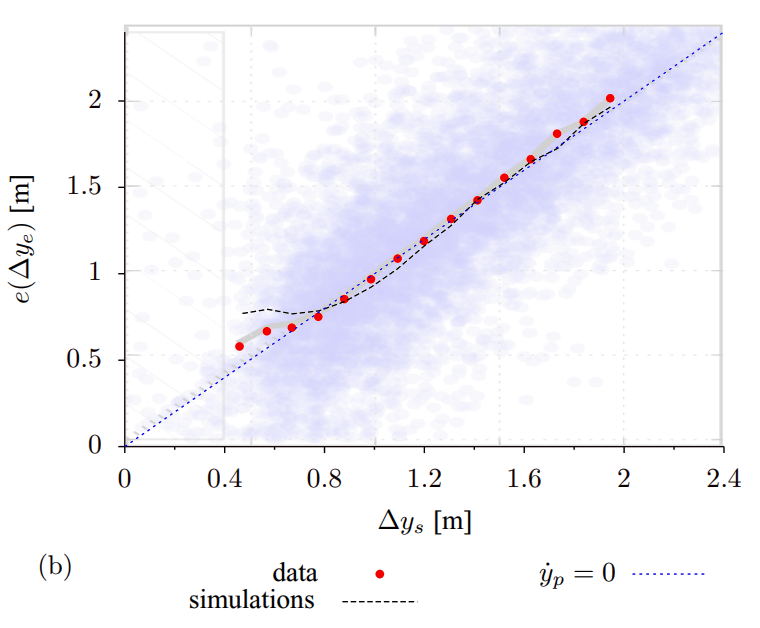
\includegraphics[width=0.4\textwidth]{images/2026-06-11-01-59-21.png}};
  \node[anchor=north, font=\small] at ($(zwei.south)+(0.3cm,+1.1cm)$) {położenie $\Delta y$ w mijaniu};
 \node[anchor=east, font=\small, rotate=90] at ($(zwei.west)+(+0.0cm,+2.1cm)$) {położenie $\Delta y$ na wyjściu};

%  \node[anchor=south] at ($(ted.south)+(-0.3cm,-3.2cm)$) {
  % równania Langevina: \usebox{\langevinbox}
%  };
\node[anchor=south east, xshift=-3mm, yshift=5mm] (eyes) at (current page.south east) {
\includegraphics[width=0.2\textwidth]{images/2026-06-10-22-42-25.png}};

 \node[anchor=east, align=right, yshift=-5mm] at (eyes.west) {\emph{\begin{tabular}{c}pan Mateusz zignorował \\ wszystkie moje zasady\end{tabular}}};

%  \caption{}
%  \end{figure}
\end{tikzpicture}
\end{frame}

\end{document}